\section{Характеристики детектора CBM RICH}\label{sec:secCbmRichOptimiz}
% \todo видимо, переделать название

Ниже представлены результаты моделирования в среде CbmRoot в связке с генератором UrQMD, выполненные (\todo не мной!) с применением актуальной геометрической модели CBM RICH, построенной с помощью ``CATIA-GDML geometry builder'' и описанной в секции~\ref{sec:chapRICHgeom}.
Результаты показывают прирост по всем показателям по сравнению с геометрией, в которой каждая фоточувствительная камера моделируется двумя плоскостями, что даёт основание полагать, что цилиндрическая форма камеры более эффективна.

В CBM RICH выработано два типовых анализа модели детектора с помощью МК моделирования. В первом анализе в геометрической установке присутствует только RICH и он обстреливается одиночными электронами из точки первичного взаимодействия с импульсом и направлением из заданного диапазона. Такой анализ позволяет оценить выход черенковских фотонов, количество регистрируемых фотонов (хитов) (см.~\figref{fig:RICHchar1}), геометрический аксептанс детектора, а также параметры восстановленных колец.

Реконструкция колец в RICH состоит из двух этапов --- поиск колец, т.е. группировка хитов, принадлежащих одному кольцу (ring finding), и фитирование, т.е. определение параметров кольца (ring fitting), причём фитирование выполняется и окружностями и эллипсами.
МК моделирование, в отличие от реального эксперимента, предоставляет полную информацию о происходящих процессах. В частности, сохраняется связь между фотонами, рождёнными от одного электрона. Это позволяет не выполнять первый этап так, как это делалось бы на реальных данных, а принять за хиты одного кольца список хитов от фотонов, рождённых от рассматриваемого электрона.
При этом второй этап индифферентен к истории хитов.
На~\figref{fig:RICHchar2} представлены распределения радиуса $R$ подобранного кольца, полуосей $A$ и $B$ подобранного эллипса. На~\figref{fig:RICHchar3} показаны распределения разброса хитов от кольца $dR$ и эллиптичности $B/A$.
Следует отметить, что в алгоритме поиска колец значение 7 выбрано как минимально допустимое количество хитов в кольце.
В случае МК моделирования с одиночными электронами возможна ситуация, когда количество хитов в кольце меньше~7 (см.~\figref{fig:RICHchar1} (справа)). Это означает, что такое кольцо теоретически есть, но не будет восстановлено.
%\todo формулировка

\begin{figure}[H]
\begin{minipage}[t]{0.495\textwidth}
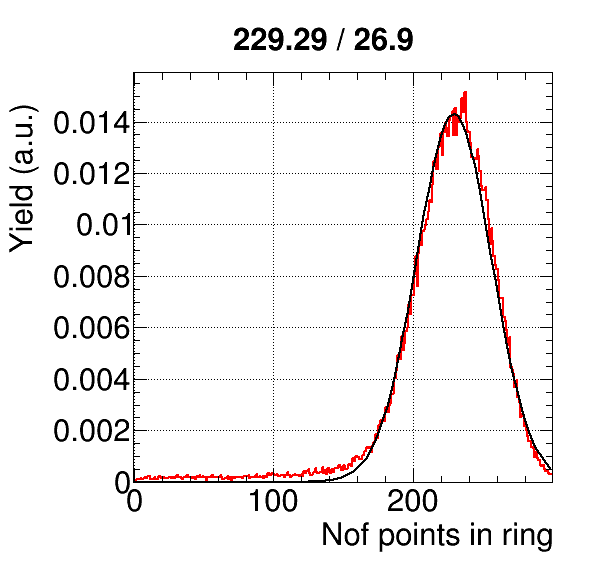
\includegraphics[width=0.9\textwidth]{pictures/RICH_nPoints_dist.png}
\end{minipage}
\begin{minipage}[t]{0.495\textwidth}
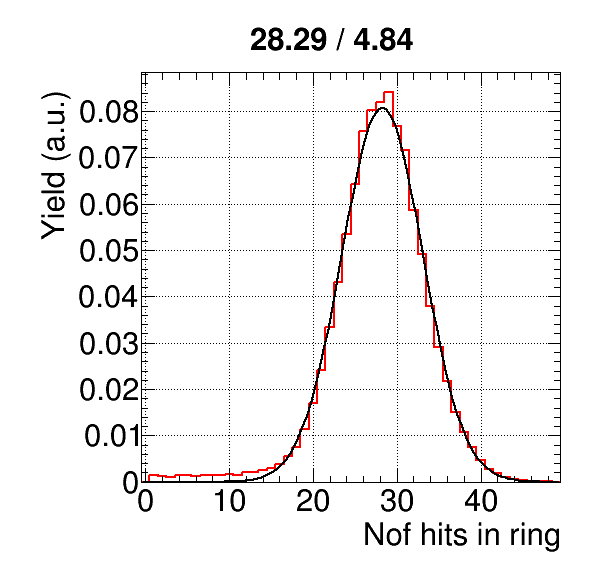
\includegraphics[width=0.9\textwidth]{pictures/RICH_nHits_dist.png}
\end{minipage}
\caption{}
\label{fig:RICHchar1}
\end{figure}

\begin{figure}[H]
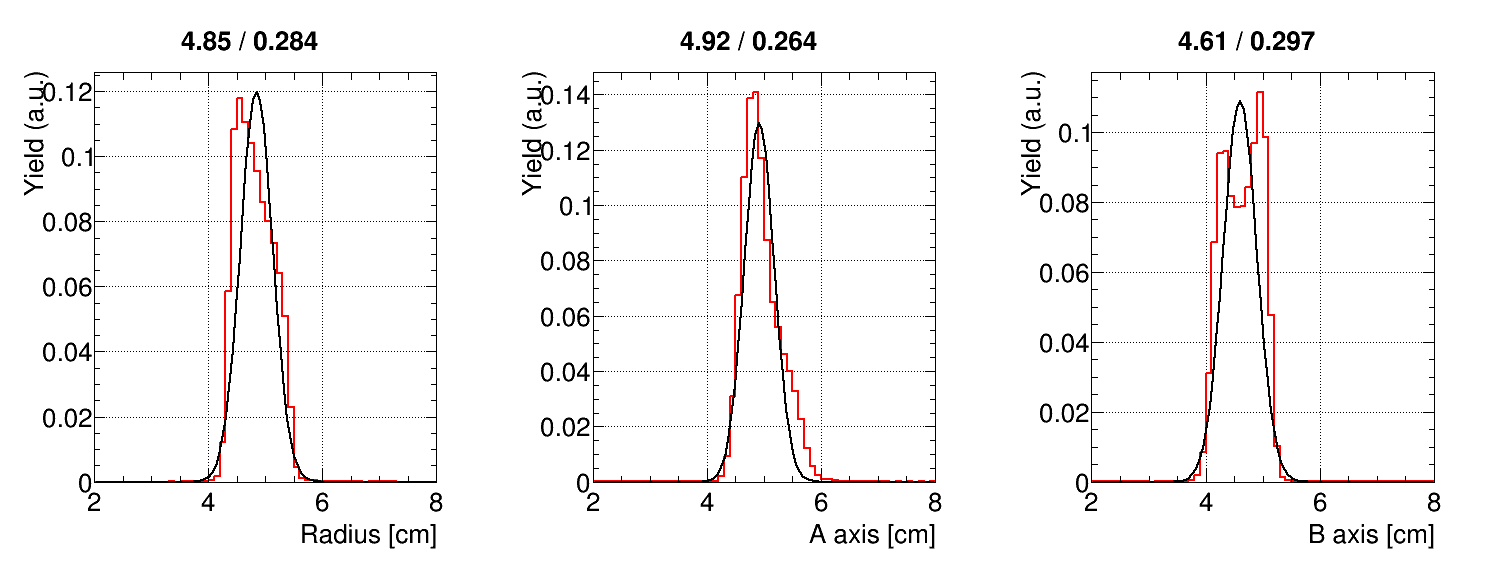
\includegraphics[width=0.95\textwidth]{pictures/RICH_R_A_B.png}
\caption{}
\label{fig:RICHchar2}
\end{figure}

\begin{figure}[H]
\begin{minipage}[t]{0.495\textwidth}
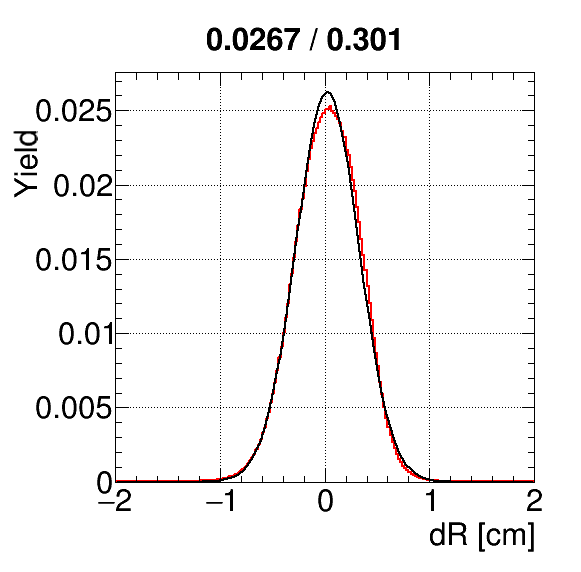
\includegraphics[width=0.9\textwidth]{pictures/RICH_dR.png}
\end{minipage}
\begin{minipage}[t]{0.495\textwidth}
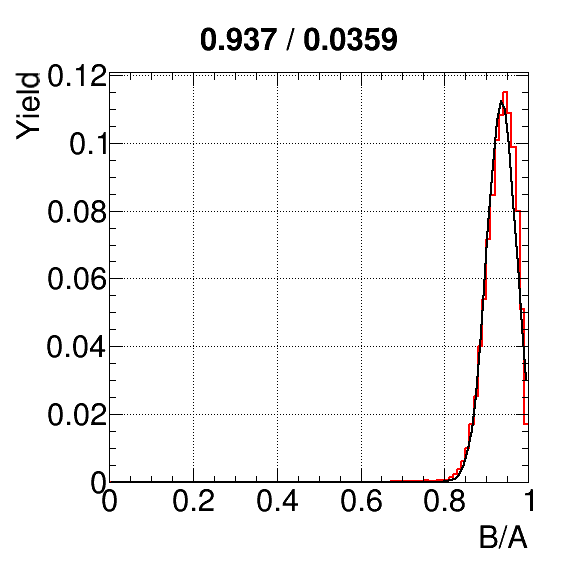
\includegraphics[width=0.9\textwidth]{pictures/RICH_BoverA.png}
\end{minipage}
\caption{}
\label{fig:RICHchar3}
\end{figure}

%Все значения - средние.
%Один электрон рождает 230 фотонов, из которых регистрируется 28 фотонов.
%Радиус кольца 4.85~см, отношение полуосей эллипсов $A/B=$0.937.


Второй анализ выполняется по результатам моделирования стандартного $Au+Au$ события CBM с помощью UrQMD. В этом случае есть две группы событий --- центральные столкновения при энергии 8~\GeVperNucl{}, характерные для SIS100, и 25~\GeVperNucl{}, характерные для SIS300.

Т.к. задача данного моделирования --- оценить функционирование детектора в реалистичной ситуации, в геометрической установке присутствуют STS и магнит. При этом присутствует магнитное поле и выполняется полная реконструкция треков в STS. На~\figref{fig:CbmRichOneEvent} представлено изображение на одной плоскости реконструкции от одного события $Au+Au$ 25~\GeVperNucl{}. Красные точки обозначают хиты, зелёные --- пересечение с плоскостью реконструкции RICH продолжений восстановленных треков STS, отражённых от зеркала.

% картинка уехала

\begin{table}[H]
\caption{}
\label{tabl:RICHAuAuChar}
\begin{tabular}{ | p{0.3\linewidth} | p{0.3\linewidth} | p{0.3\linewidth} | }
\hline
& 8~\GeVperNucl{} (SIS100) & 25~\GeVperNucl{} (SIS100) \\
\hline
$N_{hits}$ & 496 & 1431 \\
\hline
$N_{rings}$ ($\geq1$~хита) & 23.0 & 71.6 \\
\hline
$N_{rings}$ ($\geq7$~хитов) & 19.9 & 59.6 \\
\hline
\end{tabular}
\end{table}

\begin{figure}[H]
\begin{minipage}[t]{0.495\textwidth}
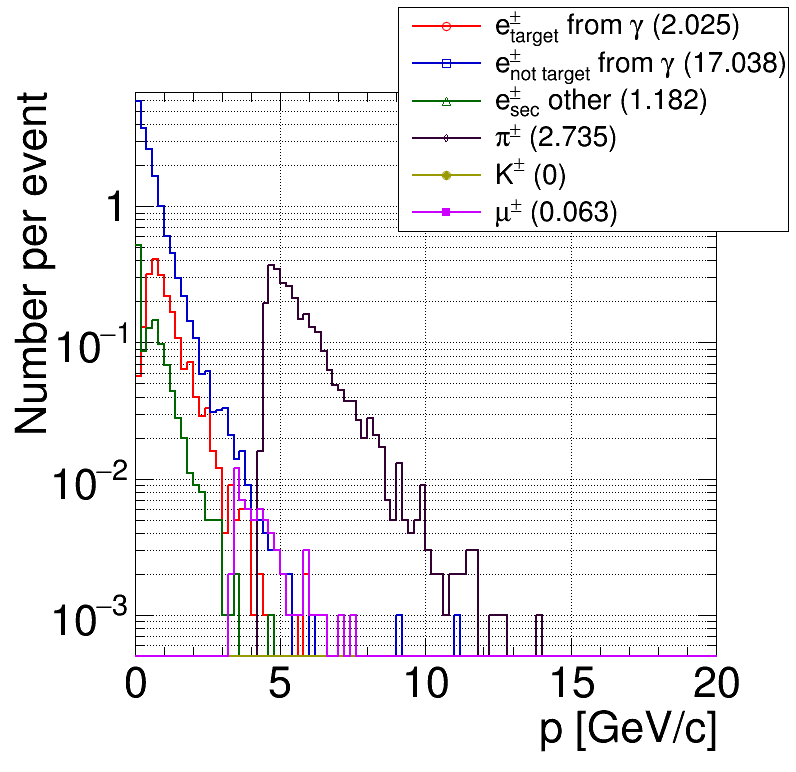
\includegraphics[width=0.9\textwidth]{pictures/RICH_8AGeV.png}
\end{minipage}
\begin{minipage}[t]{0.495\textwidth}
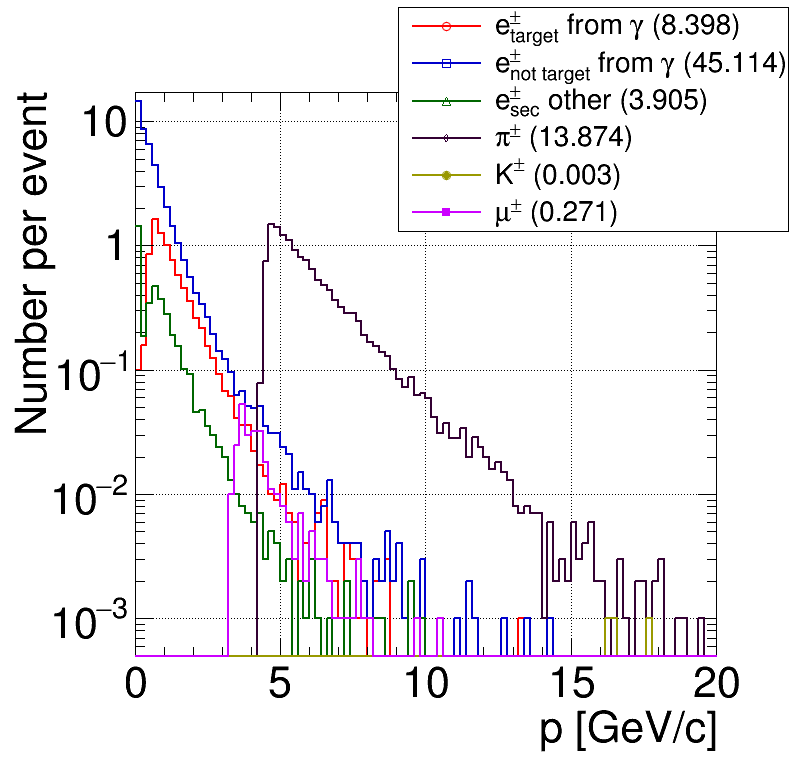
\includegraphics[width=0.9\textwidth]{pictures/RICH_25AGeV.png}
\end{minipage}
\caption{Основные типы частиц, регистрируемые в RICH при центральном $Au+Au$ столкновении при~8~\GeVperNucl{} (слева) и~25~\GeVperNucl{} (справа).}
\label{fig:RICH8and25AGeV}
\end{figure}
